\section{Introdução}

% Apresente o USV-Lab como uma plataforma da Marinha do Brasil para pesquisa e desenvolvimento em veículos autônomos marítimos.
A navegação marítima autônoma representa avanços significativos na segurança e eficiência das atividades marítimas. Embora o conceito de navios autônomos não seja recente sua aplicação atual é ampla, com benefícios como a redução de erros humanos e a otimização de recursos. No campo militar, a navegação não tripulada tem ganhado destaque, ampliando capacidades operacionais e mitigando riscos humanos. Nesse contexto, a Marinha do Brasil, com um papel estratégico na defesa da Amazônia Azul, busca desenvolver capacidades de navegação autônoma, especialmente para missões de reconhecimento, por meio do Veículo de Superfície Não Tripulado Laboratorial (VSNT-Lab), exibido na figura~\ref{fig:intro_vsnt}. Essa iniciativa reflete a estratégia da Marinha em explorar o potencial da navegação autônoma para operações táticas avançadas\cite{VSNT_douglas2024}.

\begin{figure}[H]
    \caption{Veículo de Superfície Não Tripulado Laboratorial (VSNT-Lab)}
       \centering
       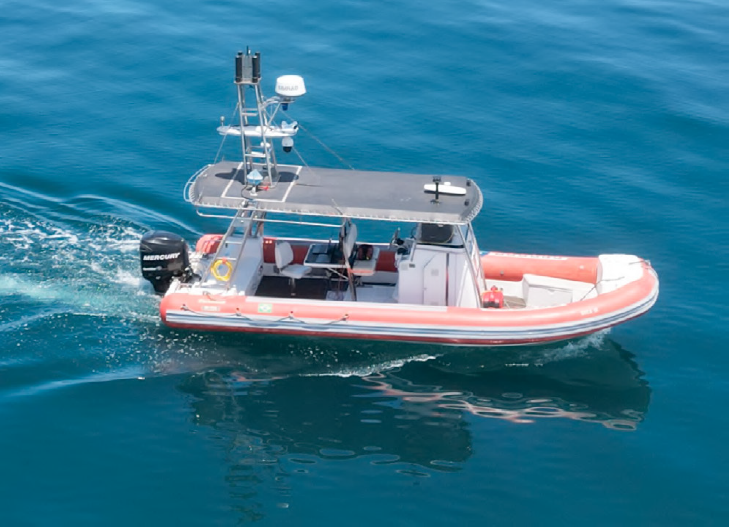
\includegraphics[height=6cm]{figuras/intro_vsnt.png}
       \label{fig:intro_vsnt}
   \small
   
   Fonte: Lima et al. \cite{VSNT_douglas2024}.
   \end{figure}

% Destaque a importância da comunicação eficiente e resiliente em missões autônomas, como as realizadas durante o exercício MINEX-23.
A comunicação híbrida do VSNT-Lab com o navio-mãe combina uma rede mesh baseada em rádio NetNode com uma conexão VPN sobre 4G, oferecendo redundância e resiliência em cenários operacionais desafiadores. Embora os autores de \cite{VSNT_douglas2024} relatem na conclusão de seu artigo que a comunicação durante o exercício MINEX-23 da Marinha do Brasil foi eficiente, as tecnologias empregadas apresentam limitações inerentes, conforme destacado em \cite{Network_alqurashi2023}. A rede mesh baseada em rádio sofre com interferências ambientais, como chuva e reflexões na superfície da água, além de seu alcance limitado, que pode comprometer a eficácia em cenários de maior extensão. Por sua vez, a conexão VPN sobre 4G depende de infraestrutura terrestre, restringindo sua aplicabilidade a áreas costeiras e tornando operações em alto-mar mais desafiadoras. Essas limitações enfatizam a necessidade de soluções híbridas mais robustas para superar os desafios de comunicação em ambientes marítimos remotos.

% Identifique problemas como latência, perda de pacotes e falhas de comunicação em canais mesh e VPN, que comprometem a autonomia e a eficiência das missões.
Os desafios de comunicação em VSNTs incluem latência, que pode impactar o controle em tempo real e a coordenação entre veículos, além de ruídos e falhas de transmissão que comprometem a confiabilidade dos dados. A largura de banda limitada é outro obstáculo, dificultando a troca simultânea de grandes volumes de informações, especialmente em comunicação de longo alcance. Esses fatores afetam diretamente a eficiência das missões, destacando a necessidade de tecnologias mais robustas e adequadas para cenários cooperativos e de alta demanda de dados\cite{VSNT_ge2018}.

% Relacione à dissertação base.
Este trabalho se inspira na metodologia apresentada por Silva\cite{Network_silva2021}, que utiliza Cadeias de Markov Ocultas (HMM) e Aprendizado por Reforço para inferir a Qualidade de Serviço (QoS) em redes de ISPs e otimizar ações de manutenção preditiva. A presente pesquisa busca adaptar e validar essa metodologia ao contexto do VSNT-Lab, considerando os desafios específicos da comunicação em veículos marítimos autônomos. Ao aplicar essas técnicas ao VSNT-Lab, espera-se aprimorar a robustez e a resiliência das comunicações em cenários críticos.

% Ressalte como a pesquisa contribui para a robustez das operações autônomas e para a segurança em missões militares e civis, alinhada aos interesses estratégicos da Marinha na "Amazônia Azul".
A pesquisa em tecnologias de comunicação para o VSNT-Lab não apenas contribui para a eficiência das operações autônomas, mas também reforça a robustez e a segurança em missões militares e civis, essenciais para os interesses estratégicos da Marinha do Brasil na defesa da Amazônia Azul. Ao enfrentar desafios como latência, perda de pacotes e falhas de comunicação, os avanços no desenvolvimento de soluções híbridas e sistemas de comunicação resilientes garantem maior confiabilidade e capacidade de resposta em cenários críticos. Além disso, essas inovações fortalecem a capacidade de monitoramento e proteção da extensa Zona Econômica Exclusiva brasileira, promovendo uma integração eficiente entre tecnologias autônomas e estratégias táticas avançadas para a soberania e a sustentabilidade no domínio marítimo.